%!TEX program = xelatex
\documentclass{article}
\usepackage[UTF8,scheme=plain]{ctex}
\usepackage[a4paper,left=1.25in,right=1.25in,top=1in,bottom=1in]{geometry}

\usepackage{amsmath,amsthm,amsfonts,amssymb}
\usepackage{graphicx}
\usepackage{float}
\usepackage{subcaption}
\usepackage{booktabs,multirow,multicol}
\usepackage{indentfirst}
\usepackage{hyperref}
\usepackage{setspace}
\usepackage{listings}
\usepackage[ruled,noline]{algorithm2e}
\usepackage{bm}
\usepackage{xcolor}

\graphicspath{
    {./figure/}{./figures/}{./image/}{./images/}{./graphic/}{./graphics/}{./picture/}{./pictures/}
}


\title{NPDE~第1次实验报告}
\author{朱浩然 PB21000234}
\date{\today}

\begin{document}

\maketitle

\section{作业要求}

函数:$$v(x) = \frac{1}{2}(\pi - x),v_N(x) = \sum_{\omega=1}^N\frac{sin(\omega x)}{\omega},x \in \Omega = (0,2\pi].$$
将$\Omega$均匀剖分$x_j=j*\Delta x$,$j=1,\cdots,m$,$\Delta x=\frac{2\pi}{m}$, 
对于$m=20$和$m=160$分别绘出$v(x)$、$v_N(x)$和$v(x)-v_N(x)$的图形。这儿$N$分别取10和100。\par 
对于修正的
$$\tilde{v}_N=\sum_{\omega=1}^N\frac{sin\frac{\omega\pi}{N}}{\frac{\omega\pi}{N}}\frac{sin\omega x}{\omega}$$
重复上面的工作;比较二者的结果,并进行评述。

\section{方法}
假设$f \in C_{(-\infty,\infty)}^{1}$是$2\pi$周期的函数,则$f(x)$可由傅里叶级数表示为:
$$f(x)=\frac{1}{\sqrt{2\pi}}\sum_{\omega=-\infty}^{\infty}\hat{f}(\omega)e^{i\omega x},$$
其中傅里叶系数$\hat{f}(\omega)$为$$\hat{f}(\omega)=\frac{1}{\sqrt{2\pi}}\int_{0}^{2\pi}f(x)e^{-i\omega x}dx,$$
且该傅里叶级数一致收敛于$f(x)$。\par
则$$v(x) = \frac{1}{2}(\pi - x)$$的傅里叶级数应为$$v_N(x) = \sum_{\omega=1}^N\frac{sin(\omega x)}{\omega}.$$\par
当存在不连续跳跃点的周期函数由傅里叶级数去表示时,在不连续的跳跃点附近会出现振荡现象,这种现象称为Gibbs现象,本问题中的函数$v(x)$正如此,具有跳跃间断点$0$与$2\pi$。
通过引入Fejér核,可以消除这种影响,Fejér核来自于对傅里叶级数进行Cesàro求和:
$$F_N(x)=\frac{D_0(x)+\cdots+D_{N-1}(x)}N=\frac1N\frac{\sin^2(\frac{Nx}{2})}{\sin^2(\frac{x}{2})}.$$
故修正后的傅里叶级数为:
$$\tilde{v}_N=\sum_{\omega=1}^N\frac{sin\frac{\omega\pi}{N}}{\frac{\omega\pi}{N}}\frac{sin\omega x}{\omega}.$$\par
根据以上原理,使用不同的$N$和$m$值,计算$v_N(x)$和$\tilde{v}_N(x)$,并比较结果。\par
文件 HW1.cpp 使用c语言编程计算,文件 HW1\underline{~}plot.m 使用MATLAB绘图。
\newpage

\section{结果}
下述结果中$v$表示原函数,$v_{10}$和$v_{100}$表示$N=10$和$N=100$时的傅里叶级数,误差图像表示$\left|v-v_{10}\right|$和$\left|v-v_{100}\right|$的差值。
\begin{figure}[htbp]
    \centering
    \begin{subfigure}[b]{0.47\textwidth}
        \centering
        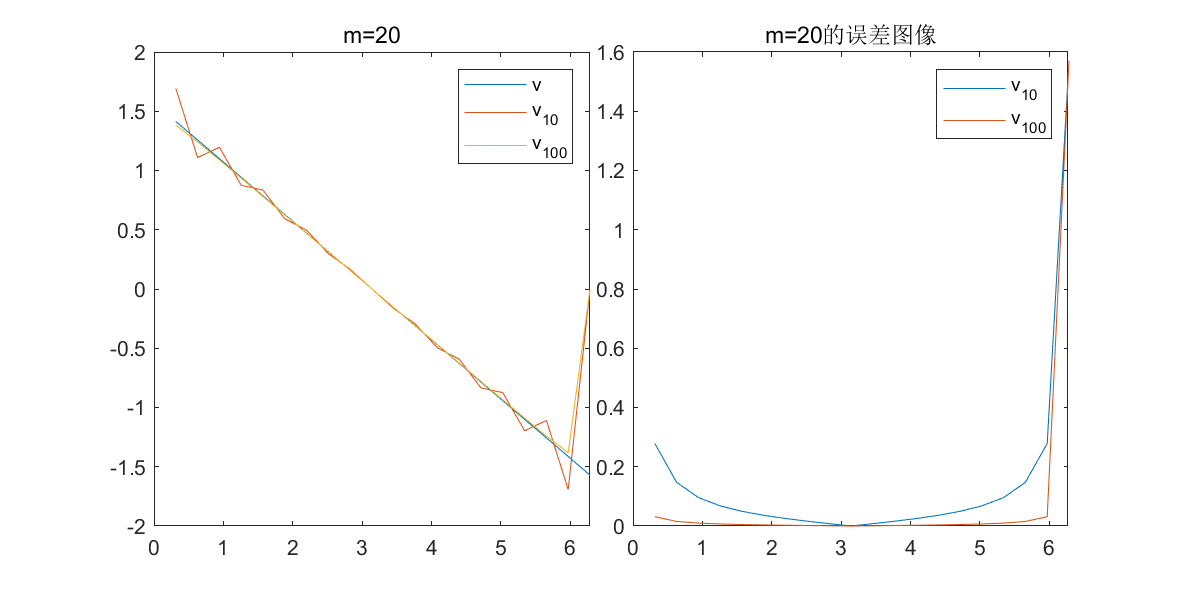
\includegraphics[width=\textwidth]{m=20.png}
        \caption{未修正}
    \end{subfigure}
    \begin{subfigure}[b]{0.47\textwidth}
        \centering
        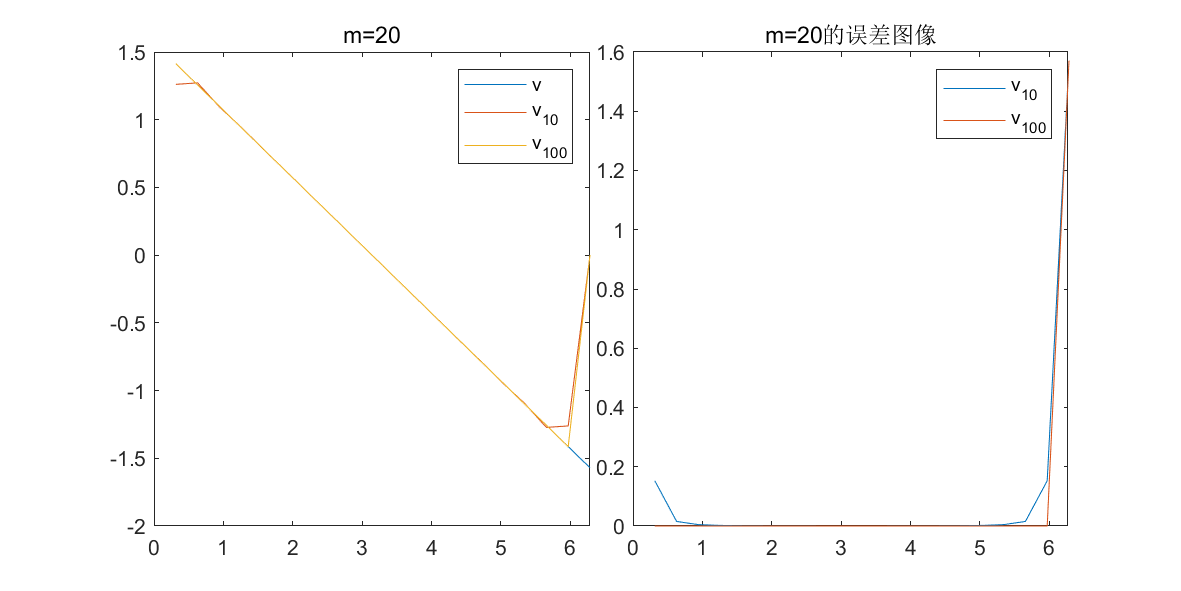
\includegraphics[width=\textwidth]{m=20修正.png}
        \caption{修正}
    \end{subfigure}
    \caption{m=20}
\end{figure}

\begin{figure}[htbp]
    \centering
    \begin{subfigure}[b]{0.47\textwidth}
        \centering
        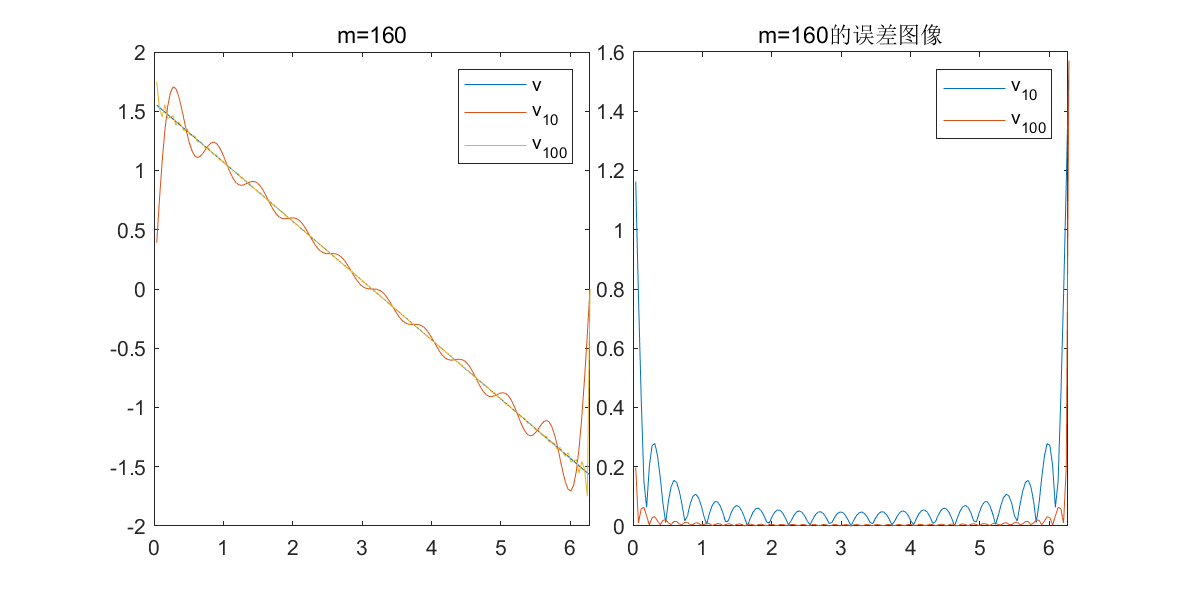
\includegraphics[width=\textwidth]{m=160.png}
        \caption{未修正}
    \end{subfigure}
    \begin{subfigure}[b]{0.47\textwidth}
        \centering
        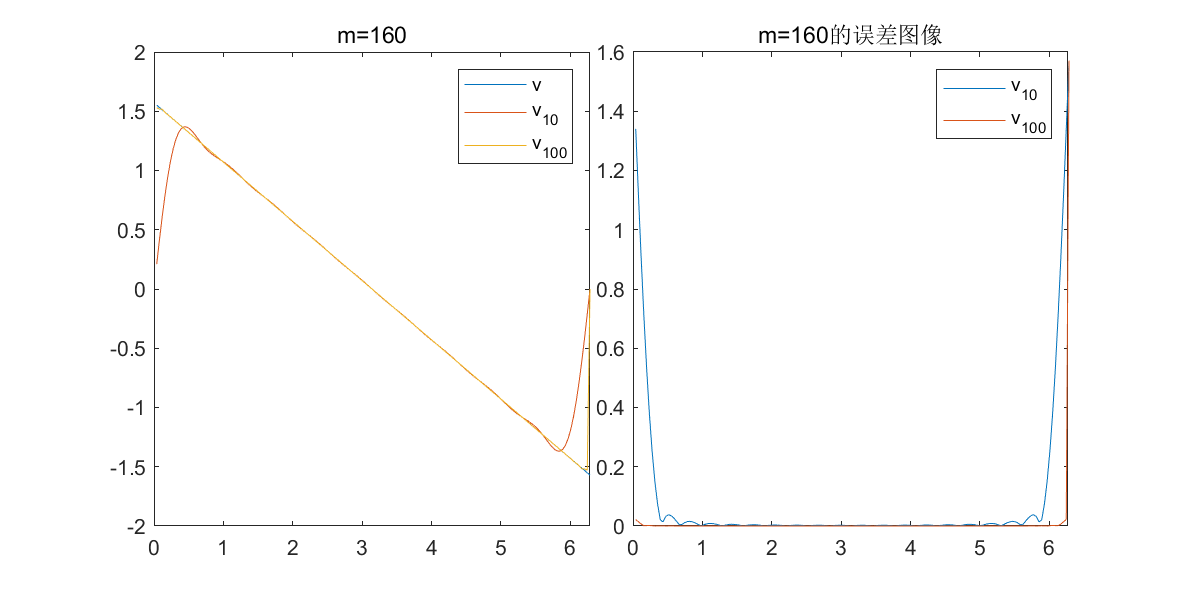
\includegraphics[width=\textwidth]{m=160修正.png}
        \caption{修正}
    \end{subfigure}
    \caption{m=160}
\end{figure}

\section{总结}
可以明显看出其他条件相同时,$N$越大,傅里叶级数逼近的误差越小。$m$的大小只影响绘图精度。
修正前的函数在$v(x)$的跳跃间断点($0$与$2\pi$)处误差最大,即发生了Gibbs现象。修正后的函数则有效消除了这种影响。

\end{document}
